The database was designed in a way that reduces redundant information to a
minimum. The structure diagram is shown in Figure \ref{fig:dbstructure} (page
\pageref{fig:dbstructure}). At the time of this writing, the tables ``ests'',
``hmmsearch'' and ``blast'' are filled in a cumulative fashion, i.e., they
contain data from all query species. This affects performance because without
administrative access to server configuration and tuning variables, a too small
InnoDB key buffer becomes a performance bottleneck \citep{mysql2013}.

% this is probably not that useful
%\input{inc/results/tab-mysql-variables}

\begin{figure}[ht]
	\centering
	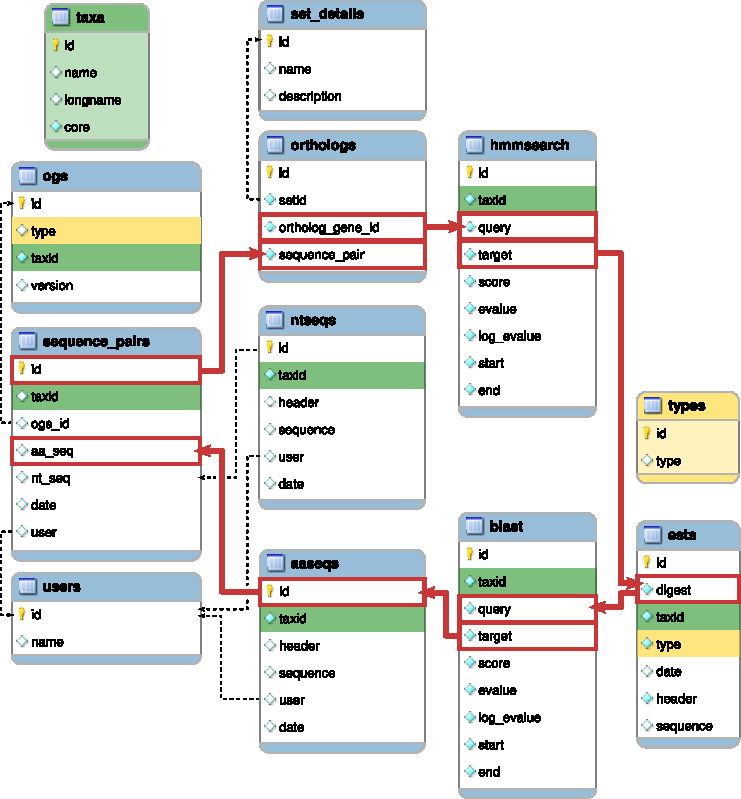
\includegraphics[width=\textwidth]{img/dbstructure.pdf}
	\caption[\pname database structure]{
		\pname database structure. Each rectangle represents a table with named
		columns. Note the circular path (red) that can be drawn across the tables and
		that is used in \code{JOIN} queries in order to construct a graph of
		orthologous relationships. Green table columns are referenced to the ``taxa''
		table, and yellow table columns are referenced to the ``types'' table. Dotted
		lines are secondary references.
	}
	\label{fig:dbstructure}
\end{figure}



